
\documentclass[12pt]{article}
\usepackage{amsmath}
\usepackage{fullpage}
\usepackage{graphicx}

\title{Shakuntala Devi: \\
PUZZLES TO PUZZLE YOU}
\author{}
\date{}

\begin{document}

\maketitle

\begin{enumerate}

\item \textbf{TALL  MEN  NEXT  DOOR} \\
Next  door  to me live four  brothers  of different  heights. Their  average  height  is 74 inches,  and the difference  in heipht  among  the  first  three  men  is two  inches. 'The difference  between  the  third  and  the  fourth  man  is six inches. 

Can you tell how  tall is each  brother? 

%
%
\item  \textbf {A  MATTER  OF  TIME} \\
Fifty  minutes  ago if it was  four  times  as many  minutes past three  o'clock,  how  many  minutes  is it until  six o'cfock? 

%
%
\item  \textbf {BROTHERS  AND  SISTERS} \\
A family  I know  has  several  children.  Each  boy  in this family  has  as many  suters  as brothers  but each  of the girls  has twice  as many  brothers  as sisters. 

How  many  brothers  and sisters  are there?

%
%
\item \textbf{AROUND  THE  EQUATOR} \\
Two identical  trains,  at the  equator  start  travelling round  the  world  in opposite  directions.  They  start  to-gether,  run  at the  same  speed  and  are  on  different tracks. 

Which  train  will  wear  out its wheel  treads  first? 

%
\item \textbf{OVER  THE  GOLDEN  GATE} \\
While  in San  Francisco  some  time  back,  I hired  a car to drive  over  the  Golden  Gate  bridge.  1 started  in the ; fternoon  when  there  was  no traffic  rush.  So  I could  do 40 miles  an hour.  While  returning,  however, I got caught  in the traffic  rush  and  I could  only  manage to drive  at a speed  of 25 miles  an hour. 

What  was  my average  speed  for the round  trip? 

%
\item  \textbf{BICYCLE  THIEVES} \\
A friend  of mine  runs  a bicycle  shop  and he narrated to me this following  story: 

A man,  who  looked  like a tourist,  came  to his shop one day  and  bought  a bicycle  from  him  for  Rs. 350. The cost  price  of the  bicycle  was  Rs.  300.  So  my friend  was  happy  that  he had  made  a profit  of Rs. 50 on the sale.  However,  at the time  of settling  the bill,  the tourist  offered  to pay  in travellers  cheques  as he had no cash money  with  him.  My  friend  hesitated.  He  had no arrangements  with  the  banks  to encash  travellers cheques.  But  he remembered  that  the  shopkeeper  next door  had such  a provision,  and so he took  the  cheques to his friend  next  door  and got cash  from  him. 

The travellers  cheques  were  made  out for Rs. 100 each and so he had taken  four  cheques  from  the tourist totalling  to Rs.  400!  On  encashing  them  my friend paid back  the tourist  the balance  of Rs. 50. 

The tourist  happily  climbed  the  bicycle  and pedalled away  whistling  a tune. 

However,  the next  morning  my friend's  neighbour,  who had taken  the  travellers  cheques  to the bank,  called  on him and returning  the cheques  which  had  proved  value-less demanded  the  refund  of his money.  My  friend quietly  refunded  the  money  to his neighbour  and tried to trace  the tourist  who  had given  him  the  bad  cheques and taken  away  his bicycle.  But  the  tourist  could  not be found. 

How  much  did my friend  lose  altogether  in this  un-fortunate  transaction? 

%
\item  \textbf{THE  DIGITS  AND  SQUARE  NUMBERS} \\
All the  nine  digits  are  arranged  here  so as to form four square  numbers: 

9, 81,  324,  576 

How  would  you  put  them  together  so as to form  a single  smallest  possible  square  number  and a single  largest possible  square  number? 

%
\item  \textbf{THE  BUS  NUMBER} \\
While  visiting  a small  town  in the  United  States,  I lost my overcoat  in a bus.  When  I reported  the matter  to the bus company  I was asked  the number  of the bus.  Though I did not  remember  the  exact  number  I did  remember that the bus number  bad  a certain  peculiarity  about  it. The number  plate  showed  the  bus number  as a perfect square  and also  if the plate  was  turned upside  dow n.? the number  would  still  be a perfect  square—of  course  it was not? 

I came  to know  from  the bus  company  they  had only five hundred  buses  numbered  from  1 to S00. 

From  this  I was  able  to deduce  the bus number. 

Can you tell what  was the other  number? 

%
\item \textbf{THE  HOUR  HAND  AND  THE  MINUTE  HAND} \\
We all know  that  the  hour  hand  and  the  minute  hand on a clock  travel  at different  speeds.  However  there  are certain  occasions  when  the hands  are exactly  opposite  each other.  

Can  you  give  a simple  formula  for calculating the times  of these  occasions? 

%
\item \textbf{TO  CATCH  A THIEF} \\
Some  time  back  while  in England  I watched  a case in a criminal  court.  A man  was  being  accused  of having stolen  certain  valuable  jewels  and  trying  to run  away with them,  when  he was caught  by a smart  police  officer who overtook  him. 

In cross  examination  the lawyer  for accused  asked  the police  officer  how  he could  catch  up with  the accused  who was already  seven  steps  ahead  of him,  when  he started  to run after  him.  'Yes  Sir.'  The  officer  replied.  'He  takes eight  steps  to every  five of mine  ! 

'But then  officer,'  interrogated  the  lawyer,  'how  did you ever  catch  him.  if that was  the case?' 

'That's  easily  explained  sir,'  replied  the officer,  *I got a longer  stride...  two  of my steps  equal  in length  to his five. So  the number  of steps  1 required  were  fewer  than his. and this  brought  me  to the  spot  where  I captured him.' 

A member  of the  jury,  who  was particularly  good  at quick  calculations  did  some  checking  and  figured  out the number  of steps  the police  officer  must  have  taken. 

Can you also  find  out  how  many  steps  the  officer needed  to catch  up with  the thief? 

%
\item \textbf{THE  GONG} \\
Supposing  a clock  takes  7 seconds  to strike  7, how long does  it take  for the same  clock  to strike  10? 

%
\item \textbf{SOMETHING  FOR  THE  MARMALADE} \\
A little  girl I know  sells  orange  from  door  to door. 

One day while  on her  rounds  she  sold  1/2 an orange more  than  half  her oranges  to the first  customer.  To  the second  customer  she sold  1/2 an orange  more  than  half  of the remainder  and to the third  and  the last  customer  she sold 1/2 an orange  more  than  half  she now  had,  leaving  her none. 

Can you tell the number  of oranges  she originally  had? Oh, by the way,  she never  had to cut an orange. 

%
\item \textbf{THE  COUNTERFEIT  NOTE} \\
While  walking  down  the street,  one  morning,  I found  a hundred  rupee  note  on the  footpath.  I picked  it up, noted  the number  and took  it home. 

In the  afternoon  the plumber  called  on me to collect his bill. As  I had no other  money  at home,  I settled  his account  with  the hundred  rupee  note  I had found.  Later I came  to know  that  the  plumber  paid  the note  to his milkman  to settle  his monthly  account,  who  paid  it to his tailor  for the garments  he had had made. 

The tailor  in turn  used  the  money  to buy  an old sewing  machine,  from  a woman  who  lives  in my  neigh-bourhood.  This  woman  incidentally,  had  borrowed  a hundred  rupees  from  me sometime  back  to buy  a pressure cooker.  She,  remembering  that  she  owed  me a hundred rupees,  came  and paid  the debt. 

I recognised  the  note  as the one I had found  on the footpath,  and on careful  examination  I discovered  that the bill was counterfeit. 

How  much  was  lost in the whole  transaction  and  by whom? 


%
\item \textbf{COTTON  OR  GOLD} \\
Which  would  you  say  is heavier,  a pound  of cotton or a pound  of gold? 

%
\item \textbf{NUTS  FOR  THE  NUTS} \\ 
Last time  I visited  a friend's  farm  near  Bangalore  he gave me a bag containing  1000  peanuts.  From  this I took out 230  peanuts  for  use  in my  own  home  and gave away  the bag with  the remainder  of peanuts  to three  little brothers  who  live  in my neighbourhood  and  told  them  to distribute  the nuts  between  themselves  in proportion  to their ages—which  together  amounted  to 17.5 years. 

Tinku,  Rinku  and  Jojo,  the  three  brothers,  divided the nuts  in the following  manner: 

As often  as Tinku  took  four  Rinku  took  three  and as often  as Tinku  took  six Jojo  took  seven. 

With  this data  can you find  out what  were  the respec-tive ages  of the boys  and how  many  nuts  each  got? 

%
\item \textbf{THE  WEDDING  ANNIVERSARY} \\
Recently  I attended  the  twelfth  wedding  anniversary celebrations  of my  good  friends  Mohini  and  Jayant. Beaming  with  pride  Jayant  looked  at his wife  and commented,  'At  the  time  we were  married  Mohini  was  3/4 of my age,  but now  she is only  5/6th. 

We began  to wonder  how  old  the couple  must  have been  each  at the time  of their  marriage! 

Can you figure  it out? 


%
\item \textbf{I'LL  GET  IT FOR  YOU  WHOLESALE...} \\
A wholesale  merchant  came  to me  one  day  and  posed this problem.  Every  day  in his business  he has to weigh amounts  from  one  pound  to one  hundred  and twenty-one pounds,  to the nearest  pound.  To  do this,  what  is the minimum  number  of weights  he needs  and how  heavy should  each  weight  be7 


\item \textbf{THE  BROKEN  GLASSES} \\
My friend  Asha  was  throwing  a very  grand  party and wanted  to borrow  from  me 100  wine  glasses.  I decided  to send  them  through  my boy servant  Harish. 

Just to give  an incentive  to Harish  to deliver  the glasses intact  I offered  him  3 paise  for every  glass  delivered safely  and threatened  to forefeit  9 paise  
for very  glass  he broke. 

On settlement  Harish  received  Rs 2.40  from  me. 

How  many  glasses  did Harish  break? 

%
\item \textbf{THE  PECULIAR  NUMBER} \\
There  is a number  which  is very  peculiar.  This  number is three  times  the sum  of its digits.  Can  you  find  the number. 

%
\item \textbf{MAKE  A CENTURY} \\
There  are eleven  different  ways  of writing  100  in tha form  of mixed  numbers  using  all the nine  digits  once  and only once.  Ten-of  the ways  have  two figures  in the integ-ral part  of the number,  but  the  eleventh  expression  has only one figure  there. 

Can you find  all the eleven  expressions? 
%
\item \textbf{THE  PERPLEXED  POSTAL  CLERK} \\ 
My friend  Shuba  works  in a post  office  and  she  sells stamps.  One  day a man  walked  in and slamming  seventy-five paise  on the counter  requested,  'Please  give  me some 2 paise  stamps,  six times  as many  one paisa  stamps,  and for the  rest  of the amount  make  up some  5 paise stamps.' 

The bewildered  Shuba  thought  for a few  moments and finally  she handed  over  the  exact  fulfilment  of the order  to the man—with  a smile. 

How  would  you have  handled  the situation? 

%
\item \textbf{THE  MYSTERY  OF THE  MISSING  PAISA} \\
Two women  were  selling  marbles  in the  market  place —one  at three  for a paise  and other  at two for a paise. One day both  of them  were  obliged  to return  home  when each had  thirty  marbles  unsold.  They  put together  the two lots  of marbles  and handing  them  over  to a friend asked  her  to sell  them  at five for 2 paise.  According  to their calculation,  after  all, 3 for one  paise  and  2 for one paise  was exactly  the same  as 5 for 2 paise. 

But when  the takings  were  handed  over  to them,  they were  both  most  surprised,  because  the entire  lot together had fetched  only  24 paisel  If however,  they  had  sold their marbles  separately  they  would  have  fetched  25 paise. 

Now  where  did  the  one  paise  go? Can  you explain the mystery? 

%
\item \textbf{WALKING  BACK  TO HAPPINESS} \\
A man  I know,  who  lives  in my  neighbourhood, travels  to Chinsura  every  day  for his work.  His  wife drives  him  over  to Howrah  Station  every  morning  and in the evening  exactly  at 6 P.M.  she  picks  him  up back  at the station  and takes  him home. 

One day  he was  let off at work  an hour  earlier,  and so he arrived  at the Howrah  Station  at 5 P.M.  instead  of at 6. He  started  walking  home.  However  he met  wife enroute  to the  station  and  got into  the car. They drove  home  arriving  10 minutes  earlier  than  usual. 

How  long  did  the  man  have  to walk,  before  he was picked  up by his wife? 
%
\item \textbf{ON  THE  LINE} \\
It is a small  town  railway  station  and  there  are  25 stations  on that  line.  At  each  of the  25 stations  the passengers  can  get  tickets  for  any  of the  others  24 stations. 

How  many  different  kinds  of tickets  do you  think the booking  clerk  has to keep? 
%
\item \textbf{THE  LEGACY} 
When  my  unclc  in Madura  died  recently,  he left  a will, instructing  his executors  to divide  his estate  of Rs. 1,920,000  in this  manner:  Every  son should  receive  three times  as much  as a daughter,  and  that  every  daughter should  get twice  as much  as their  mother. 

What  is my aunt's  share? 
%
\item \textbf{THE  ROUND  TABLE} \\
We have  a circular  dining  table  made  of marble which  has  come  down  to us as a family  heirloom.  Ws also have  some  beautiful  bone-china  saucers  that  I recently  brought  from  Japan. 

Our table  top  is fifteen  times  the  diameter  of our saucers  which  are also  circular.  We  would  like to place the saucers  on the table  so that  they  neither  over  lap each other  nor the edge  of the table. 

How  many  can we place  in this manner?
%
\item \textbf{DOWN  THE  ESCALATOR} \\
Recently,  while  in London,  I decided  to walk  down the escalator  of a tube  station.  I did some  quick  cal-culations  in my  mind.  I found  that  if I walk  down twenty-six  steps,  I require  thirty  seconds  to reach  the bottom.  However,  if I am able  to step  down  thirty-four stairs  I would  only  require  eighteen  seconds  to get to the bottom. 

If the  time  is measured  from  the  moment  the top step begins  to descend  to the time  I step  off the last  step at the bottom,  can  you  tell  the  height  of the stairway in steps? 
%
\item \textbf{THE  CHESS  BOARD} \\
We all know  that  a chess  board  has  64 squares.  This can be completely  covered  by 32 cardboard  rectangles, each cardboard  covering  just 2 squares.

Supposing  we remove  2 squares  of the chess  board  at diagonally  opposite  corners,  can  we cover  the modified board  with  31 rectangles?  If it can  be done  how  can we do it? And  if it cannot  be  done,  prove  it impossible. 
%
\item \textbf{THE  GAME  OF CATS  AND  MICE} \\
A number  of cats  got  together  and  decided  to kill between  them  999919  mice.  Every  cat  killed  an equal number  of mice. 

How  many  cats  do you think  there  were? 

Oh, by the  way  let me  clarify  just two  points—it  is not one cat killed  the lot, because  I have  said  'Cats'  and it is not-999919  cats  each  killed  one mouse,  because  I have used the word  'mice'. 

I can  give  you  just  one  clue—each  cat killed  more mice  than  there  were  cats. 
%
\item \textbf{THE  WHEELS} \\
A friend  of mine  in Bangalore  owns  a horse-driven carriage.  It was  found  that  the fore  wheels  of the carriage make  four  more  revolutions  than  the hind  wheel  in going 96 feet.  However,  it was  also  found  that  if the circum-ference  of the fore  wheel  were  3/2 as great  and of the hind wheel  4/3 as  great,  then  the fore  wheel  would  make  only 2 revolutions  more  than  the hind  wheel  in going  the same distance  of 96 feet. 

Can you find  the circumference  of each  wheel? 
%
\item \textbf{BLOW  HOT  BLOW  COLD} \\
It is a matter  of common  knowledge  that  0C  is the same  as 32F.  It is also  a known  fact  that  100C  equals 212F.  But  there  is a temperature  that  gives  the same reading  on both  Centigrade  and Fahrenheit  scales. 

Can you find  this temperature? 
%
\item \textbf{THE  LLAMA  RACE} \\
Recently,  while  I was  in a holiday  resort  in Peru  I watched  a very  interesting  spectacle.  Two  gentlemen  by the name  of Sr. Guittierez  and Sr. Ibanez  decided  to have a Llama  race  over  the  mile  course  on the beach  sands. They  requested  me and some  of my  other  friends  whom I had met at the resort  to act as the judges.  We  stationed ourselves  at different  points  on the  course,  which  was marked  off in quarter  miles. 

But, the two Llamas,  being  good  friends  decided  not to part  company,  and ran together  the whole  way.  How-ever,  we the  judges,  noted  with  interest  the  following results: 

The Llamas  ran  the  first  three  quarters  in six and three  quarters  minutes.  They  took  the  same  time  to run the first half mile  as the second  half.  And  they  ran the third  quarter  in exactly  the  same  time  as the last quarter. 

From  these  results  I became  very  much  interested  in finding  out  just  how  long  it took  those  two  Llamas  to run the whole  mile. 

Can you find  out the answer? 
%
\item \textbf{THE  SHATTERED  CLOCK} \\
A clock  with  the  hours  round  the  face  in Roman block  numerals,  as illustrated  in the sketch fell down,  and  the  dial  broke  into  four  parts.  The numerals  in each  part  in every  case  summed  to a total of 20. 

Can you  show  how  the four  parts  of the  clock  face was broken? 

\begin{figure}[h]
\begin{center}
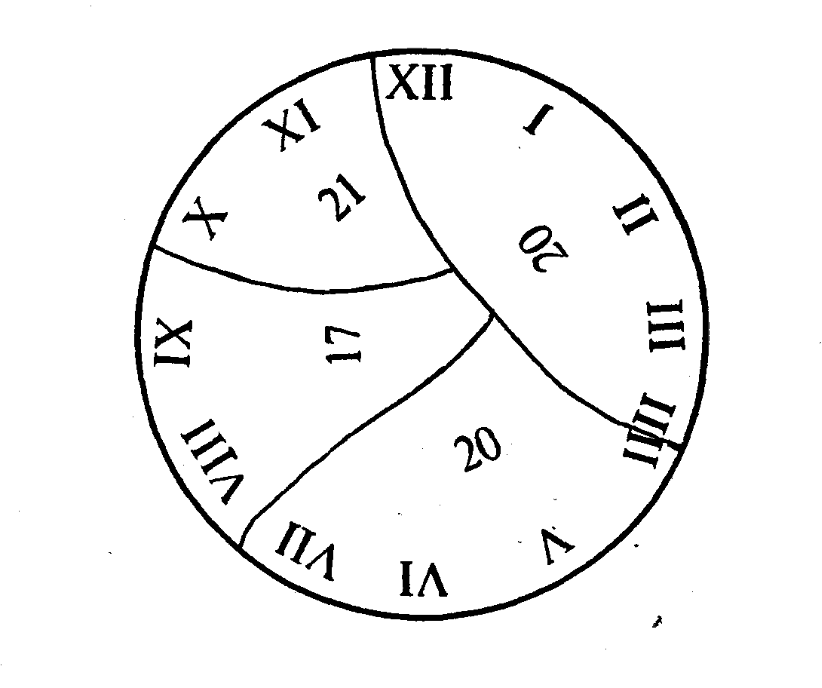
\includegraphics[width=0.5\textwidth]{sdevi_q33.png}
\caption{ Qs 33}
\end{center}
\end{figure}

%
\item \textbf{THE  PAINTED  WINDOW} \\
My room  has  a square  window  of 4 feet  across  and  4 feet down.  I decided  to get  only  half  the area  of the window  painted.  Even  after  the painting  I found  that the clear  part  of the window  still remained  a square  and still measured  4 feet from  top to bottom  and 4 feet  from side to side. 

How  is it possible? 
%
\item \textbf{ANIMALS  ON  THE  FARM} \\
My friend  who  owns  a farm  near  Bangalore  has  five droves  of animals  on his farm  consisting  of cows,  sheep and pigs  with  the  same  number  of animals  in each drove. 

One day he decided  to sell them  all and sold  them  to eight  dealers. 

Each  of the eight  dealers  bought  the same  number  of animals  and  paid  at the  rate  of Rs. 17 for  each  cow, Rs. 2 for each  sheep  and Rs. 2 for each  pig. 

My friend  recieved  from  the  dealers  in total  Rs. 301. 

How  many  animals  in all did he have  and  how  many of each  kind? 
%
\item \textbf{WHICH  IS THE  BETTER  BARGAIN?} \\
Recently  while  shopping  in New  Market  in Calcutta, I came  across  two very  nice  frocks  selling  at a discount. I decided  to buy  one  of them  for my little  girl Mammu. The shopkeeper  offered  me one of the  frocks  for Rs.  35 usually  selling  for 8/7 of  that  price  and the other  one for 
Rs. 30 usually  selling  for  7/6 of that  price. 

Of the two frocks  which  one do you think  is a better bargain  and by how  much  per cent? 
%
\item \textbf{WALKING  ALL  THE  WAY} \\
One day I decided  to walk  all the  way  from  Bangalore to Tumkur.  I started  exactly  at noon.  And  someone  I know  in Tumkur  decided  to walk  all the way  to Bangalore from  Tumkur  and  she  started  exactly  at 2 JP.M.,  on the same  day. 

We met  on the  Bangalore-Tumkur  Road  at five past four,  and we both  reached  our destination  at exactly  the same  time. 

At what  time  did we both  arrive? 
%
\item \textbf{THE  TRAIN  AND  THE  CYCLIST} \\
A railway  track  runs  parallel  to a road  until  a bend brings  the road  to a level  crossing.  A cyclist  rides  along to work  along  the road  every  day at a constant  speed  of 12 miles  per hour. 

He normally  meets  a train  that  travels  in the same direction  at the crossing. 

One day he was late by 25 minutes  and  met  the  train 6 miles  ahead  of the level  crossing.  

Can  you  figure  out the speed  of the train? 
%
\item \textbf{SOMETHING  FOR  PROFIT} \\
A friend  of mine  bought  a used  pressure  cooker  for Rs. 60. She  somehow  did not find  it useful  and so when a • friend  of hers  offered  her Rs. 70 she sold  it to her. However,  she felt bad after  selling  it and decided  to buy it back  from  her  friend'  by offering  her Rs.  80. After having  bought  it ooce  again  she felt that she did not really need the  cooker.  So  she  sold  it at the  auction  for Rs. 90. 

How  much  profit  did she make?  Did  she  at all make any profit? 
%
\item \textbf{THE  DIGITAL  GAME} \\
There  is a number,  the second  digit  of which  is smaller than its first  digit  by 4, and if the  number  was  divided  by the digits  sum,  the quotient  would  be 7. 

Can you find  the number? 


\item \textbf{THE  NUMBER  AND  THE  SQUARE} \\
\begin{figure}[h]
\begin{center}
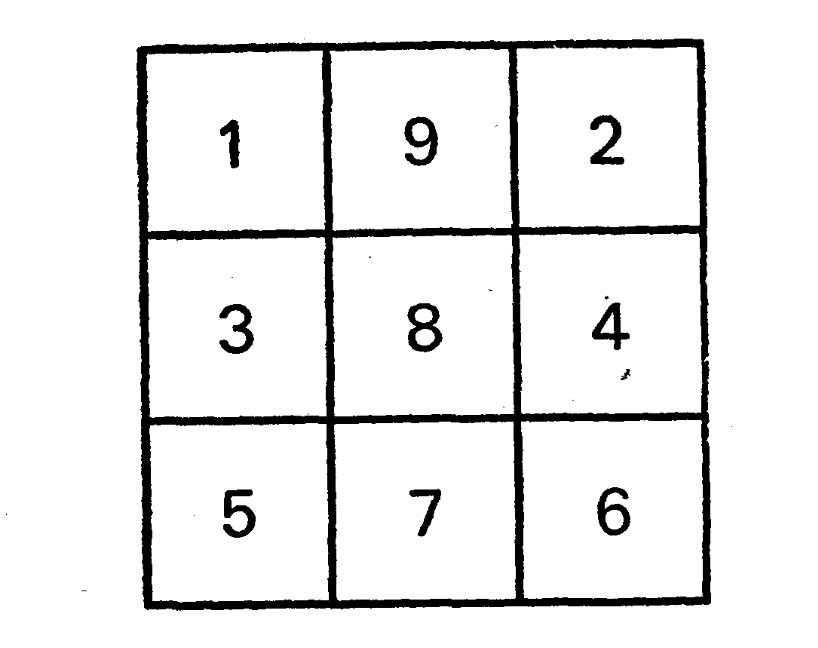
\includegraphics[width=0.5\textwidth]{sdevi_q41.png}
\caption{ Qs 41}
\end{center}
\end{figure}
In the  diagram  above  the  numbers  from  I to 9 are arranged  in a square  in such  a way  that the number  in the second  row is twice  that in the first  row  and  the  number in the bottom  row  three  times  that  in the top row. 

I am told  that  there  are three  other  ways  of arranging the numbers  so as to produce  the same  result. 

Can you find  the other  three  ways? 
%
\item \textbf{THE  FAULTY  MACHINE} \\
A factory  manufacturing  flywheels  for racing  cars  has ten machines  to make  them.  The  manufacturer  knows the correct  weight  for a flywheel. 

However,  one day  one  of the machines  begins  to pro-duce  faulty  parts—either  overweight  or underweight. 

How  can the manufacturer  find  the faulty  machine  in only two weighings? 
%
\item \textbf{SQUARES  AND  RIGHT  ANGLES} \\
Can you  make  2 squares  and  4 rightangled  triangles using  only  8 straight  lines? 
%
\item \textbf{THE  DISHONEST  MERCHANT} \\
An unscrupulous  trader  decided  to make  some  extra profit  oo Coffee.  He  bought  one type  of coffee  powder  at Rs. 32 a kilo  and mixed  some  of it with  a better  quality of coffee  powder  bought  at Rs.  40 a kilo,  and he sold the blend  at 43 a kilo.  That  gave  him  a profit  of 25 per cent  on the cost. 

How  many  kilos  of each  kind  must  he use to make  a blend  of a hundred  kilos  weight? 
%
\item \textbf{FOR  THE  CHARITIES} \\
One day when  I was  walking  on the road  in New  Delhi, a group  of boys  approached  me  for donation  for their poor  boys'  fund.  I gave  them  a rupee  more  than  half the money  I had in my purse.  I must  have  walked  a few more  yards  when  a group  of women  approaphed  me  for donations  for an orpbange.  I gave  them  two  rupees  more than half  the  money  I had  in my purse.  Then,  after  a few yards  I was  approached  by a religious  group  for a donation  to the temple  they  were  building.  .1 gave  them three  rupees  more  than  half of what  I had in my purse. 

At last when  returned  to my hotel  room,  I found  that I had only  one rupee  remaining  in my purse. 

How  much  money  did  I have  in my  purse  when  I started? 
%
\item \textbf{THE  NUMBER  GAME} \\
The product  of three  consecutive  numbers  when  divi-ded by each  of them  in turn,  the sum  of the three  quo-tients  will be 74. 

What  are the numbers? 
%
\item \textbf{THE  SARI  AND  THE  BLOUSE} \\
I bought  ft sari  and  a blouse  for Rs.  110 at the New *Market.  The  sari  cost  Rs.  100 more  than  the blouse, how much  does  the sari cost? 
%
\item \textbf{WHEN  WAS  HE BORN?} \\
Some  months  back,  this  year,  I was  waiking  through the Central  Park  in New  York. 

I saw  an intelligent  looking  little  boy  playing  all by himself  on the grass.  I decided  to talk  to him  and  just as an excuse  to start  the  conversation  I asked  him  his age. A mischivious  glint  flickered  in his eyes  and he replied,  'Two  days  back  I was  ten years  old, and next  year I shall  be thirteen.  If you know  what's  today  you'll  be able to figure  out  my  birthday  and  that'll  give  you my age.'  I looked  at him bewildered. 

How  old was the boy? 
%
\item \textbf{THE WEIGHT  OF THE  BLOCK}\\
A cement  block  balances  evenly  in the scales  with  three quarters  of a pound  and three  quarters  of a block.  

What is the weight  of the whole  block.  / 
%
\item \textbf{LUCRATIVE  BUSINESS} \\
Two unemployed  young  men  decided  to start  a business together.  They  pooled  in their  savings,  which  came  to Rs 2,000.  They  were  both  lucky,  their  business  pros-pered  and  they  were  able  to increase  (heir  capital  by 50 per cent  every  three  years. 

How  much  did they  have  in all at the end of eighteen years. 
%
\item \textbf{THE  OLD  SHIP} \\
Some  years  back  I was  travelling  by a cargo  ship  from New Zealand  to Tahiti.  I was curious  to look  around  the ship one day and in the boiler  room  I asked  a man  how old the ship  was.  He  smiled  and replied  me in this  way: 'The ship  is twice  as old as its boiler  was when  the ship was as old as the boiler  is now.  And  the  combined  age of the ship  and the boiler  is thirty  years.' 

Can you  figure  out what  is the age of the ship  and of the boiler? 
%
\item \textbf{THE  THREE  CONTAINERS} \\
We have  three  containers  which  hold  19, 13 and  7 ounces  of liquid  respectively.  The  19 ounce  container  is empty  but the 13 and 7 ounce  containers  are full.  

How can we measure  out  10 ounces  by using  only  the three above  mentioned  containers? 
%
\item \textbf{ON  THE  WAY  TO MARKET} \\
One morning  I was on  my way  to the market  and met  a man coming from the market who had 4 wives.  Each  of the  wives  had  4 bags containing  4 dogs  and each  dog had 4 puppys. 

Taking  all things  into  consideration  how  many  were going  to market? 
%
\item \textbf{A  MATTER  OF  DENOMINATOR} \\
A fraction  has the denominator  greater  than  its numerator by 6. But  if you add 8 to the denominator,  the value  of the fraction  would  then  become  1/3.

Can you  find  this fraction? 
%
\item \textbf{RIGHT  FOOT  FORWARD} \\
A short  man  takes  three  steps  to a tall man's  two  steps. They  both  start  out on the left foot.  

How  many  steps  do they have  to take  before  they  are both  stepping  out on the right  foot  together? 
%
\item \textbf{A  PROBLEM  OF SOCKS} \\ 
Mammu  wears  socks  of two  different  colours—white and brown.  She  keeps  them  all in the same  drawer  in a state of complete  disorder. She has altogether  20 white  socks  and 20 brown  socks in the drawer.  

Supposing  she has to take  out the socks  in the dark,  how  many  must  she take  out of the drawer  to be sure  that she has a matching  pair? 
%
\item \textbf{A  FAIR  DIVISION}\\ 
A rich farmer  died  leaving  behind  a hundred  acres  of his farm  to be divided  among  his three  daughters  Rashmi, Mala  and  Rekha—in  the  proportion  of one-third,  cne-fourth  and one-fifth  respectively/  But  Rekha  died  unex-pectedly. 

Now  how  should  the executor  divide  the land  between Rashmi  and Mala  in a fair  manner? 
%
\item \textbf{HEADS  I WIN  TAILS  I LOOSE} \\
Durisg  my last visit  to Las Vegas  in the U.S.A.,  I met  a man who  was an inveterate  gambler.  He  took  out  a coin from  his pocket  and said  to me, 'Heads  I win,  tails  I loose. I'll bet half  the money  in my pocket.' 

He tossed  the coin,  lost and gave  me half the money  in his pocket.  He  repeated  the bet again  and again  each  time offering  half  the money  in his pocket. 

The game  went  on for  quite  some  time.  I can't  re-collect  exactly  how  long  the game  went  on or how  many times  the coin  was  tossed,  but  I do remember  that  the times  he lost was exactly  equal  to the  number  of times that he won. 

What  do you  think,  did  he, on the  whole,  gain  or loose? 
%
\item \textbf{MATHEMATICS  AND  LITERATURE} \\
Recently  a publishing  company  which  specialises  in mathe-matical  books,  advertised  the job opening  of an assistant editor.  The  response  was  good.  One  hundred  people applied  for the position.  The  company,  however,  wanted to make  their  selection  from  the applicants  who  had  some training  in both  mathematics  and literature. 

Of the one hundred  applicants  the company  found  that 10 of them  had  had  no training  in mathematics  and no training  in literature.  Seventy  of them  had  had  some mathematical  training  and 82 had had some  in literature. 

How  many  applicant  shad  had training  in both  mathe-matics  and literature? 
%
\item \textbf{PROBLEM  FROM  LILAVATI} \\ 
Here  is an ancient  problem  from  Bhaskaracharya's Lilavati: 

Beautiful  maiden,  with  beaming  eyes,  tell me which  is the number  that,  multiplied  by 3, then  increased  by three-fourths  of the product,  divided  by 7, diminished  by one-third  of the  quotient,  multiplied  by itself,  diminished  by 52, the  square  root  found,  addition  of 8, division  by 10 gives  the number  2? 

Well,  it sounds  complicated,  doesn't  it? No,  not if you know  how  to go about  it. 
%
\item \textbf{UP THE  LADDER} \\ 
A man  wafts  to reach  up a window  40 ft. from  the ground. The distance  from  the foot  of the ladder  to the wall  is 9 feet. 

How  long  should  the ladder  be? 
%
\item \textbf{PIGS  AND  DUCKS} \\
While  driving  through  the  countryside  one  day I saw a farmer  tending  his pigs  and ducks  in his yard.  I was  cu-rious  to know  how  many  of each  he had.  I stopped  the car and inquired. 

Leaning  on the  stile  jovially,  he replied,'I  have  alto-gether  60 eyes  and 86 feet between  them.'

I drove  off trying  to calculate  in my mind  the  exact number  of ducks  and pigs  he had. 

What  do you think  is the answer? 
%
\item \textbf{THE  EGG  VENDOR  AND  HIS  EGGS} \\
Rasool,  the man  who  delivers  eggs  to my home  everyday, did not  turn  up one  day.  So  when  he came  the next morning  I demanded  an explanation  from  him.  He  told me the following  story: 

The previous  morning  when  he just  came  out  of the house  carrying  a basketful  of eggs  oh his head  to start  his daily  rounds  and  stepped  on to the  street,  a car going full speed  brushed  against  him  and  knocked  down  his basket  destroying  all the  eggs.  The  driver,  however,  a thorough  gentleman  admitted  his responsibility  and offered to compensate  him  for'damages.  But  Rasool  could not remember  the exact  number  of eggs  he had,  but  he estimated  the  number  at between  50 and 100.  He  was also able  to tell the gentleman  that  if the eggs  were  counted by 2's and 3's at a time,  none  would  be left,  but if counted by S's at a time,  3 would  remain,  and that  he sold  the eggs at SO paise  a piece.  ' 

The gentleman  made  some  quick  calculations  and paid Rasool  adequately. 

How  much  did the gentleman  pay Rasool? 
%
\item \textbf{SOME  LUCK!} \\
A society  of farmers  who  own  farms  in the vicinity  of my home  town  Bangalore,  planned  on holding  a raffle and persuaded  me to buy a ticket.  The  value  of the ticket was Rs. 5. As  I did not want  to pay  the entire  amount myself,  I asked  my friend  Radha  to chip  in with  me,  and offered  to share  with  her in proportion  the prize  bounty— if there  was  going  to be any.  She  paid  Rs. 2 and  I paid the rest. 

As luck  would  have  it—Bingo!...  we won  the first prize—a  flock  of 50 sheept  Good  God!...  Niether  of us knew  what  to do with  the sheep...  Where  would  we take them  in the first  place?  Neither  of us had had any  train-ing as shepherds!  So  we decided  to sell the sheep  back to the farmers. 

As per  our  original  understanding  20 of the  sheep belonged  to Radha  and 30 were  mine. However,  I decided  that  we had won  the prize  because of our  combined  luck,  and  so we should  divide  its value equally. The sheep—30  of mine  and 20 of Radha's—were  sold, each at the same-price,  and I paid  her  Rs.  150  to make the sum  equal. 

What  was  the value  per sheep? 
%
\item \textbf{THE  FAULTY  WATCH} \\
One day  I found  a strange  thing  happening  to my watch—the  minute  hand  and the hour  hand  were  coming together  every  sixty-five  minutes.  I decided  to have  it seen to. 

Was my watch  gaining  or losing  time,  and  how  much per hour? 
%
\item \textbf{THE  TRAINS  AND  THE  FALCON} 
Two trains  start  towards  each  other  from  two stations SO miles  apart,  at the same  time  and  on a single  track. Just when  the trains'  start  out,  a falcon  leaves  the first train and flies  directly  to the other  train,  and as soon  as it reaches  the second  train,  the bird  starts  back  towards  the first train.  It continues  doing  so, flying  backwards  and forwards  from  one  train  to the  other  until  the trains meet. 

Both  the trains  travel  at a speed  of 25 miles  per  hour, and the bird  flies  at 100  miles  per hour. 

How  many  miles  will the falcon  have  flown  before  the trains  met? 

\item \textbf{WHICH  IS MORE  LUCRATIVE?} \\ 
A businessman  advertised  two  job openings  for peons  in his firm.  Two  men  applied  and the businessman  decided to engage  both  or them.  He  offered  them  a salary  of Rs. 2,000  per  year;  Rs. 1,000  to be paid  every  half  year,  with a promise  that  their  salary  would  be raised  if their  work proved  satisfactory.  They  could  have  a raise  of Rs. 300 per year,  or if they  preferred,  Rs.  300  each  half year. 

The two  men  thought  for  a few  moments  and then one of them  expressed  his wish  to take  the  raise  at Rs 300 per  year,  while  the  other  man  said  he would  accept the half yearly  increase  of Rs. 100. 

Between  the two men,  who  was the gainer,  and by how much? 
%
\item \textbf{LITTLE  MAMMU  AND  THE  MARBLES} \\
Little  Mammu  was  playing  marbles  with  her friend  Nawal I heard  her say to him,  'if you give  me one of your  marbles I'll have  as many  as you.'  Nawal  replied,  'you  give  me one of your  marbles,  and  I'll  have  twice  as many as you.' 

I wondered  how  many  marbles  each  had!  What  do you think? 
%
\item \textbf{A FAMILY  MATTER} \\
Fifteen  years  back  my neighbour  Mrs.  Sareen  had  three daughters  Sudha,  Seema  and Reema—and  their  combined ages were  half of hers.  During  the  next  five years  Sonny was born  and Mrs.  Sareen's  age equalled  the total  of all her children's  ages. 

After  some  years  Kishu  was  born  and then  Sudha  was as old  as Reema  and  Sonny  together.  And  now,  the combined  age of all the children  is double  Mrs.  Sareen's age, which  is, as a matter  of fact,  only  equal  to that  of Sudha  and Seema  together.  Sudha's  age is also  equal  to that of the two sons. 

What  is the age of each  one of them? 
%
\item \textbf{THE  HIGH-RISE} \\
While  in Canada,  I visited  a beautiful  hjgh-rise  building in the  Metropolitan  City  of Toronto.  The  manager of the  building  told  me  that  the  building  consisted  of different  kinds  of apartments  large  and small.  Two  room apartments  were  5\%  in number,  2.5's—7\%  in number, 3's—15\%  in number,  3.5s—20\%  in number,  4.5s—49\% in number,  5's—33\%  in number,  5.5's—12\%  in number, 6's—3\%  in number  and in addition  several  4 room  apart-ments.  Altogether  the  building  contained  437  apart-ments. 

Can you  figure  out how  many  apartments  are there  in eacb type,  using  round  figures? 
%
\item \textbf{THE  CURIOUS  LICENSE  PLATE}
When  I acquired  my Mercedes-Benz  car in Germany,  the first thing  I had  to do was  to get a license  plate.  The plate  I got had a peculiar  number  on it. It consisted  of 5 different  numbers  and by mistake  when  I fixed  it upside down  the number  could  be still read,  but  the  value  had increased  by 78633. 

What  was  my actual  license  number? 
%
\item \textbf{LOOSE  OR GAIN} \\ 
A man  I know  runs  a workshop  in Calcutta.  He  bought two lathes  to use  in his workshop.  However,  he found out afterwards  that  they  did  not  serve  the purpose  for which  he had  bought  them,  and  so he decided  to sell them.  He  sold  them  each  for  Rs. 600 making  a loss of 20\%  on one  of them  and  a profit  of 20\%  on the other. 

Did he lose  or gain  in the transaction,  and  how  much did each  machine  cost  him? 
48 
%
\item \textbf{ON THE  SEE-SAW} \\
Some  days  back,  walking  through  the  park,  I saw  a little  girl  trying  play  the see-saw  all by herself.  It take two to see-saw,  but  here  was  a girl  who  was ingenious enough  to try and see-saw  on her own. I saw  her trying  a number  of bricks  to one end of the plank  to balance  her weight  at the other. I curiously  noted  that  she just balanced  against  sixteen bricks,  when  these  were  fixed  to the short  end of the plank and I also  noticed  that  if she were  to fix them  to the  long end of the plank,  she only  needed  eleven  as balance. 

I wondered  what  was  the  girl's  weight.  The  brick, I could  guess  weighed  equal  to a three  quarter  brick  and three  quarters  of a pound. 

Can you figure  it out? 
%
\item \textbf{A  PROBLEM  OF  COMBINATION} \\ 
A box  contains  12 marbles  of three  different  colours gTeen,  yellow  and blue—4  each. 

If you  were  to close  your  eyes  and pick  them  at ran-dom,  how  many  marbles  must  you  take  out to be sure that there  are  at least  two  of one  colour  among  the marbles  picked  out 
%
\item \textbf{THE  SPECIAL  NUMBER} \\ 
There  is a number  whose  double  is greater  than  its half by 45. 

Can you  find  this number? 
%
\item \textbf{SAWING  THE  TREE  TRUNK} \\
A heavy  tree  trunk  can  be sawed  into  a piece  12 ft long in one minute.

How  long  will it take  to saw it into  twelve equal  pieces? 
%
\item \textbf{THE  BIGAMIST} 
A man  I know  in Bombay  committed  bigamy,  by marrying two women  at brief  intervals,  one without  the knowledge of the  other.  Somehow  he was  not  brought  to the notice  of the law and  though,  if exposed  the axe could fall on him  any day,  he decided  to get the best  out of the situation  while  it lasted. 

He was  fond  of both  the  women  and had no special preference  for either.  One  lived  near  Churchgate  and the other  in Bandra.  He  worked  near  a station  midway between  Churchgate  and Bandra. 

After  work  he generally  went  to the station,  and took whichever  train  got into  the station  first—Churchgate  or Bandra.  He  arrived  at whichever  his destination  it wast at random  times,  but  found  that  be was  visiting  his Churchgate  wife  much  more  often  than  the other,  despite the fact  that both  the Churchgate  and  Bandra  trains  were on schedules  which  brought  him  to hiS  station  equally often.  Since  the same  thing  had  been  happening  for a very long  time,  chance  has  been  ruled  out  as the reason. 

Can you  find  the  reason  for  the  frequency  of his Churchgate  trips? 
%
\item \textbf{THE  SPLIT} \\
Can you split  34. parts  intp  two parts  such  that 4/7 of one 
of the parts  equals 2/5 of  the other? 
%
\item \textbf{AT  THE  FETE} \\
A number  of us went  out together  to a charity  fete  one day. Our  party  consisted  of 4 different  professional groups,  namely  25 writers,  20 doctors,  18 dentists  and  12 bank  employees.  We  spent  altogether  Rs. 1,330. 

Later  it was  found  that  five writers  spent  as much  as four doctors,  that twelve  doctors  spent  as much  as nine dentists,  and  that  six dentists  spent  as much  as eight  bank employees. 

How  much  did  each  of the four  professional  groups spend? 
%
\item \textbf{AT THE  STORE} \\
I entered  a store  and spent  one-half  of the money  that  was in my  purse.  When  I came  put I found  that  I had  just as many  paise  as I had rupees  and half  as many  rupees  as I had paise  when  I went  in. 

How  much  money  did I have  on me when  I entered? 
%
\item \textbf{THE  COUNTERFEIT  COINS} \\ 
During  my last visit  to the U.K.  I spent  a few  days  in a small  town,  where  I stayed  as a paying  guest  with  a British landlady.  The  heaters  in the  rooming  house  were  all coin operated. 

One day my landlady  requested  my help  in sorting  out a problem. 

There  were  one  hundred  and  twenty  coins  in her gas-meter  and one of them,  she knew,  was  counterfeit.  The counterfeit  coin  was  either  heavier  or lighter  than  the others.

Now  the problem  was  to isolate  this  counterfeit  coin and find  out  whether  it was  lighter  or heavier,  in five weighings. 

How  can one do it? 

\item \textbf{MULTIPLYING  BACTERIA} \\
Bacteria  is known  to multiply  very  rapidly. 

A certain  container  contains  just  one bacteria  on the first day and there  are twice  as many  on the next  day.  In this manner  the number  of bacteria  in the  container doubles  itself  everyday. 

Assuming  that  the  container  would  be full of bacteria on the 10th  day,  on which  day  would  the  container  be half full. 


\item \textbf{THE  MATHEMATICAL  SHEPHERD} \\
Shepherd  Gopal  had  a curious  aptitude  for mathematics and he was known  around  where  he lived  as the 'Counting Shepherd'. 

A man  passing  through  the  meadow  one  day  saw Gopal  grazing  a number  of sheep  and in the course  of a short  cpnversation  asked  him  how  many  of the grazing sheep  were  his own.  Gopal's  reply  absolutely  baffled  him, which  was  as follows: 

'If you  divide  my sheep  into  two gifferent  parts,  the difference  between  the  two  numbers  will  be the same  as the difference  between  their  squares. Npw  figure  it out for yourself  the number  of sheep  I own.' 

Can you say just how  many  sheep  Gopal  had? 
%
\item \textbf{A PUZZLING  NUMBER} \\
There  is a number  which  is greater  than  the  aggregate  of its third,  tenth  and the twelfth  parts  by 58. 

Can you find  the number? 
%
\item \textbf{WHAT  A COINCIDENCE?} \\
A group  of seven  young  men  named  Arun,  Binoy,  Chun-der, Dev,  Edward,  Fakruddin  and  Govind  were  recently engaged  in a game.  They  had  agreed  that  whenever  a player  won  a game  he should  double  the money  of each of the  other  players,  in other  words  he was to give  the players  just as much  money  as they  had  already  in their pockets. 

In all they  played  seven  games  and,  strangely,  each won a game  in turn  in the order  in which  their  names  are given.  But  what  was  even  more  strange  was  that  when they had finished  the game  each  of the seven  young  men had exactly  the same  amount,  Rs. 32 in his pocket. 

Can you find  out how  much  money  each  person  had with him  before  they  began  the game? 
55 
%
\item \textbf{THE  IDLER} \\
Ram  Rakhan  was  well-known  all around  his neighbour-hood  for being  a very  lazy  person.  So  when  he went around  looking  for a job as a farm-hand  everyone  refused to engage  him,  except  farmer  Gulab  Singh,  who  was a very smart  person. 

Gulab  Singh  engaged  the services  of Ram  Rakhan  at a salary  of Rs. 240 a month  consisting  of 30 days.  How-ever,  he set a condition  that  he would  forefeit  Rs. 10 a day for everyday  that  he idled.  Ram  Rakhan  accepted the job. 

At the  end  of the  month  it was  found  that  neither owed  the other  anything.  This  tought  a lesson  to Ram Rakhan. 

Can you tell jusf how  many  days  Ram  Rakhan  worked and how  many  days  he idled?

%
\item \textbf{NUMBERS  GAME} \\ 
During  one of my tours  to Canada,  I came  across  a very interesting  gam*  participated  by two players. 

A group  of match  sticks  is placed  on the table  and then it is reduced  in turn  by each  player  by removing  from the group  at least  1 but not more  than  4 match  sticks. 

The player  who  takes  the  last  match  stick  is the winner. 

If there  is a group  of 17 match  sticks  on the table  how would  you  make  your  first  move,  if it was  your  turn  and how would  you continue  to play  to win? 
%
\item \textbf{FATHER  AND  SON} \\
A father,  I know,  is 4 times  his  son's  age.  And  in 30 years  the son will be half as old as his father. 

How  old are the father  and son each  n*w? 
%
\item \textbf{A  BARGAIN  IN GUAVAS} \\
Recently.  I bought  some  guavas  at New  market  for Rs> 1.20.  Bat  they  were  so small  that  I made  the vendor throw  in two extra  guavas  for the samfe  price. 

As I began  to walk  away  the vendor  mumbled  that this transaction  had made  him lose  10 paise  a dozen  less the price  we had settled. 

How  many  guavas  did I get for my Rs. 1.20? 
%
\item \textbf{THE  SIX  MATCHES} \\
Shown  in the sketch  are six matchsticks 

\begin{figure}[h]
\begin{center}
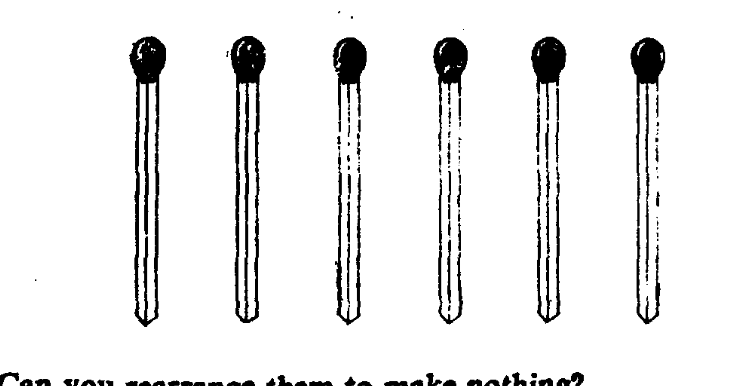
\includegraphics[width=0.5\textwidth]{sdevi_q90.png}
\caption{ Qs 90}
\end{center}
\end{figure}

T T T T T T
Can you  rearrange  them  to make  nothing? 
%
\item \textbf{NO CHANGE  PLEASE!} \\
I bad Rs. 1.15  in my purse  in 6 coins,  but I found  that  I could  not  give  change  for a rupee,  nor of a half  rupee, quarter  rupee,  ten paise  or five paise. 

Which  6 coins  did I have? 
%
\item \textbf{A  DATE  TO RECKON  WITH} \\
The date  8.8.64,  meaning  August  8, 1964  is a very  interes-ting date,  because  the  product  of the first  two numbers equals  the third. 

Can you find  the year  of the twentieth  century  which gives  the greatest  number  of occasions  of this kind? 
%
\item \textbf{GOLD  FOR  ALL  OCCASIONS} \\ 
Which is worth  more,  a bucket  full of half  a sovereign gold pieces  or an identical  bucket  full of 1 sovereign  gold pieces? 
%
\item \textbf{THE  INK-SPOT} \\
One day,  Mammu,  home  from  school  set a very  interes-ting problem  to me.  She  pushed  a large  circular  table we have  at home,  into  the corner  of the room,  so that  it touched  both  walls  and  spilled  a spot  of ink  on the extreme  edge,  and she said,  'Mummy  here  is a little  puzzle for you.  Look  at that  spot.  It is exactly  eight  inches from  one wall  and nine  inches  from  the other,  Now  tell me the diameter  of the table  without  measuring  it.

Can you? 
%
\item \textbf{SPADE  FOR  A HEART} \\ 
Here  is a spade:

\begin{figure}[h]
\begin{center}
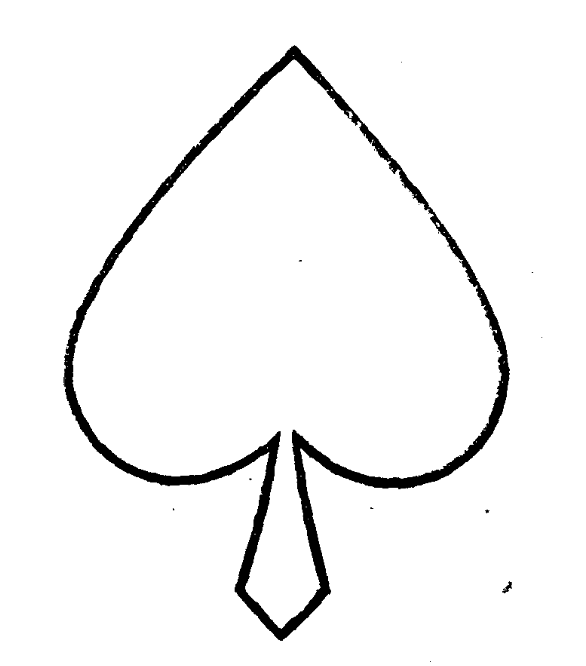
\includegraphics[width=0.4\textwidth]{sdevi_q95.png}
\caption{ Qs 95}
\end{center}
\end{figure}

Can you cut the spade  into  three  pieces  that  will  fit to-gether  and form  a heart? 

Remember,  no part  of the material  should  be wasted. 
%
\item \textbf{THE  NUMBER  PUZZLE} \\
There  are  two  numbers  with  the difference  of 3 between them  and  the difference  of their  squares  is 51. 

Can you  find  the numbers? 
%
\item \textbf{A  PROBLEM  OF COINS} \\ 
Can you  place  10 coins  in such  a way  that  they  lie in 5 straight  lines  and on each  line  there  are 4 coins. 

There  are at least  two  solutions. 
%
\item \textbf{THE  SQUIRREL  AND  THE  POST} \\
I saw  a squirrel  climbing  up a cylindrical  post  spirally, making  the circuit  in four  feet. 

Supposing  the  top  of the post  is sixteen  feet high  and three  feet  in circumference,  how  many  feet doe*  it travel to the top? 
%
\item \textbf{HEARTS  APART} \\
A man  I know  fell  in love  with  a woman  who  lived  63 miles  away.  Finally  he decided  to propose  marriage  to his beloved  and invited  her to travel  towards  his place  and offered  to meet  her on route  and bring  her home. 

The man  is able  to cover  4 miles  per  hour  to the woman's  3 miles  per hour. 

How  far will each  have  travelled  upon  meeting?
%
\item \textbf{THE  CURFEW} \\
In most  States  in India  the  law for the sale  of alcoholic beverages  provides  that  beer  cannot  be sold  after  a certain hour.  However,  in some  States  the law permits  a custo-mer to consume,  after  the deadline,  what  has  been  sold before  the curfew. 

In a certain  bar 2 men  ordered  sufficient  beer  to cover their probable  requirements  in anticipation  of the  curfew. One man  ordered  and  paid  for  5 bottles  and the other man ordered  and  paid  for 3 bottles.  But  as the  curfew sounded,  an old  friend  of both  the men  approached  and requested  them  to share  with  him  the  drinks.  The  two man agreed  and shared  the total  eight  bottles  of beer  between  them. T

he friend  thanked  the two men  and  put  down  Rs. 8 in payment  for the beer  he had consumed,  asking  them  to share  the money  in proportion  to the quantity  of beer  they have  contributed  to him. 

How  should  this money  be equitably  divided  between the two men?
%
\item \textbf{A  PROBLEM  OF AGE} \\
Recently  I met a woman  I hadn't  seen  in a long  time.  In the course  of conversation  she said,  'Do  you know  some-thing  funny?  If you reverse  my own  age,  the figures  repre-sent my husband's  age.  He is of course  senior  to me and the difference  between  our ages  is one-eleventh  of their  sum. 

Can you find  out the woman's  age as well  as her hus-band's  age? 

\item \textbf{THE  CIRCULAR  NUMBERS} \\
Here  is a sketch: 

\begin{figure}[h]
\begin{center}
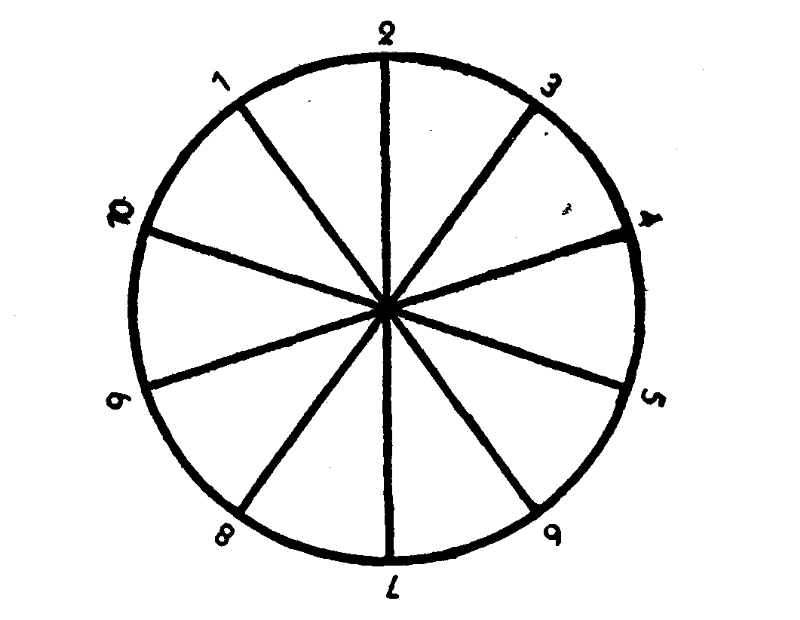
\includegraphics[width=0.5\textwidth]{sdevi_q102.png}
\caption{ Qs 102}
\end{center}
\end{figure}

Can you rearrange  the position  of the  numbers  1 to 10 so that  the sum  of any two  adjacent  numbers  is equal to the sum  of the pair of numbers  at the opposite  ends  of the diameters? 


\item \textbf{THE  PASSENGER  TRAIN AND  THE  GOODS  TRAIN} \\
Two trains,  a passenger  train  and  a goods  train  are running  in the same  direction  on parallel  railway  tracks. The passenger  train  takes  three  times  as long  to pass  the goods—even  when  they  are  going  in the  opposite directions. 

If the trains  run at uniform  speeds,  how  many  times faster  than  the  freight  train  is the  passenger  train moving? 


\item \textbf{RICE  FOR  THE  FESTIVAL} \\ 
At a certain  festivity  a rich  man  decided  to distribute free rice to deserving  people.  He  had  altogether  100 kilos  of rice  and  he wanted  to distribute  the  grain  to 100 people  in such  a manner  that  each  old person  received three  kilos,  each  youiig  person  two  and each  child  half  a kilo.  

How  many  old persons,  young  persons  and children were  there? 
%
\item \textbf{THREES  TO MAKE  THIRTY-ONE} \\
Can you write  31 using  only  the digit  3 five times? 
%
\item \textbf{SWARM  OF BEES} \\
Here  is another  problem  from  Bhaskaracharya's  Lilavati: 

The square  root  of half  the  number  of bees  in a swarm  has flown  out upon  a jasmine  bush;  eightninths  of the whole  swarm  has remained  behind;  one  female  bee flies about  a male  that  is buzzing  within  the  lotus  flower into which  he was allured  in the night  by its sweet  odour, but is now  inprisoned  in it. Tell  me  the  number  of bees? 


\item \textbf{WHAT  WERE  YOU  DOING WHEN  THE  LIGHTS  WENT  OUT?} \\
Last time  there  was  load  shedding  in Calcutta,  I was reading  a very  interesting  book  and I could  not stop.  My neighbour  Parveen  gave  me two candles  and  assured  me that I could  manage  with  them. 

Though  the candles  were  of the same  length,  Parveen told me that  one candle  would  burn  for  four  hours  and the other  for five hours. 

After  I had been  reading  for some  time  1 put the candles  out as the lights  came  on again.  And  I noticed that what  remained  of one candle  was  exactly  four  times the length  of what  was  left of the other. 

Can you find  out just  how  long  those  two  candles were  burning? 
%
\item \textbf{THE  DOTTED  SQUAKE} \\

\begin{figure}[h]
\begin{center}
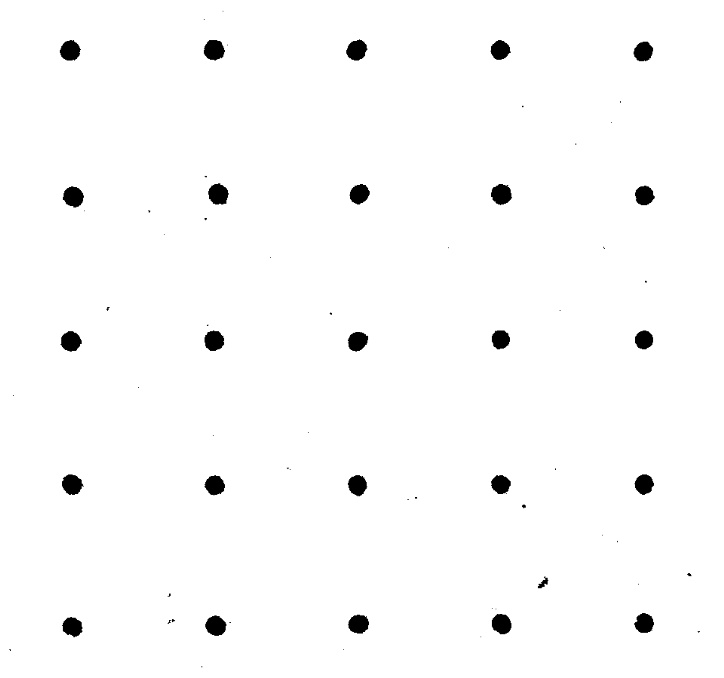
\includegraphics[width=0.5\textwidth]{sdevi_q108.png}
\caption{ Qs 108}
\end{center}
\end{figure}

Twesty-Sve  dot*  arc arranged  in a square  formation 
ra S rows  of 5, as shows  ia the sketch: 

Can you  connect  12 of these  dots  with  straight  fees to form  a perfect  cross  which  has five dots  iaaido  it and 8 dots outside? 
%
\item \textbf{STORY  OF  THE  THREE  FARMERS} \\ 
Three  farmers  paid  Rs.  1,000  for  a small  pasture. One farmer  grazed  his 9 mules,  another  his 12 cows  for twice  the time  and the last  man  put  in some  goats  for 2£ times  as the second  man's  cows  and paid  half  the  cost of the pasture. 

Can you find  out how  many  goats  did  the  last  man have,  if 6 cows  eat as much  as 4 mules,  and  10 goats  as much  as 3 cows  ? And  how  much  did the first  and  second man each  pay? 
%
\item \textbf{UP  THE  STREAM—DOWN  THE  STREAM} \\
While up stream, a crew can row a boat in eight andmfour-sevenths minutes. But if there were no stream they could row it in seven minutes less than it takes them to drift down the stream.

Can you say how long it would take them to row down with the stream?
%
\item \textbf{STAFF  AND  THE  STEEPLE} \\ 
A five feet long  staff  casts  a shadow  2 feet  long.  Can you find  the  height  of a steeple  whose  shadow  at the same  hour,  is 120 ft. long? 
%
\item \textbf{WINE  AND  WATER} \\ 
While  I was  talking  to a chemist  one  day,  he set me this interesting  problem: 

'I decided  to mix some  wine  spirits  and water.  I had two bottles  containing  10 ounces  of each.  I poured  just a quarter  of an ounce  of spirits  into  the water  and  shook them  up. You  can see clearly  that  the mixture  was  forty to one.  Now  I thought  that  I should  have  the  same quantity  of fluid  in both  the bottles,  and so I poured  back a quarter  of an ounce  of the  mixture  into  the  bottle containing  water.'  < 

Can you tell what  proportion  of spirits  to water  did the spirits  of wine  bottle  then  contain? 

\item \textbf{THE  LONG  TUNNEL} \\
A train  is one  mile  long.  It travels  at the  rate  of one mile  a minute  through  a tunnel  which  is also  one mile long. 

Can you say how  long  it will take  for the train  to pus completely  through  the tunnel? 

\item \textbf{THE  HORSE,  THE  COW  AND  THE  SHEEP} \\ 
A man  owns  a horse,  a cow  and  a sheep.  He  also owns  a pasture  to graze  them  all. 

If the  horse  and  cow  can  eat  the  contents  of the pasture  in 40 days,  while  the horse  and sheep  can  do it in 60 days  and the cow  and the sheep  in 90 days,  how long should  it take  all of them  eating  together? 

\item \textbf{THE  TWO  MATHEMATICAL  MEN} \\ 
In Bangalore  there  i* a well  known  Science  Institute. During  a visit  I asked  two of the  men  to tell me their ages.  One  replied,  'One  of our ages  subtracted  from  tke other's  equals  30.' 

Then  the other  man  spoke,  'Our  ages  multiplied  together  equal  1624'. 

What  were  their  ages? 
%
\item \textbf{A  QUESTION  OF MILEAGE} \\
If 5 litres  were  used  on a car  which  hat  travelled 20,000  miles,  how  many  miles  did eack  litre  sustain,  if aU the litres  were  used  equally  in sustaining  this mileage? 
73 
%
\item \textbf{A  PROBLEM  OF  DISSECTION} \\ 
The shape  shown  in the  sketch  below,  obviously,  is that of a square  attached  to half  of another  similar  square, divided  diagonally: 

\begin{figure}[h]
\begin{center}
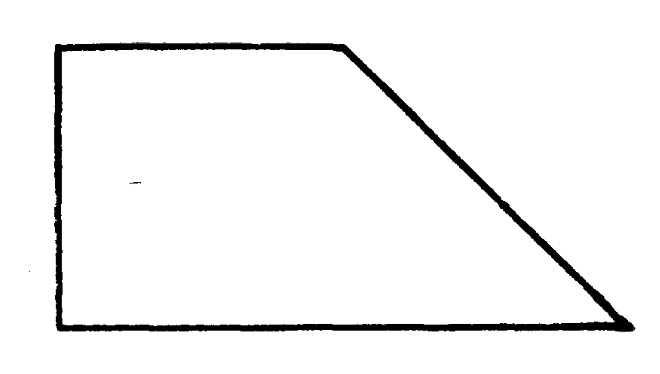
\includegraphics[width=0.5\textwidth]{sdevi_q117.png}
\caption{ Qs 117}
\end{center}
\end{figure}


Can you divide  it into  four  pieces  all of precisely  the same  size and shape? 
%
\item \textbf{THE SIXTEEN  FOURS} \\ 
How  can  you  make  a total  of 1,000  by using  sixteen 4's ? 

\item \textbf{THE STRANGE  TWO  NUMBERS} \\
There  are  two  whole  numbers,  whose  difference  of their squares  is a cube  and the  difference  of their  cubes is a square.  These  are the  smallest  possible  numbers. 

Can you  find  the numbers? 


\item \textbf{HOW MUCH?} \\
I have  two 10 paise  coins.  If 4/5 of  what  I have  is 8/9
of what  you have,  how  much  do you have? 

\item \textbf{THE MIXED  DOUBLE} \\ 
Four  married  couples  played  a tennis  tournament  of 'mixed  doubles'.  A man  and  a woman  always  played against  a man  and a woman.  However,  no person  ever played  with  or against  any other  person  more  than  once. They  all played  together  in two courts  on three  successive days. 

Can you show  how  they  could  have  done  it? 


\item \textbf{THE  BARGAIN} \\
Sometimes  one  is mystified  at the startling  reductions some  people  make  in their  prices  and  wonders  on what principle  the reductions  are based.  To  quote  an example three  years  ago a friend  offered  me a used  typewriter  for Rs. 1024.  A  year  later  he offered  me the  same  for Rs. 640  and last year  he wanted  Rs.  400  and  now  he is willing  to sell  it to me  for Rs.  250.  But  I have decided  to buy it when  he reduces  next  time. I

f he does  a consistent  reduction,  at what  price  will he offer  the typewriter  to me next? 


\item \textbf{AT  THE  FAIR} \\
At the  fair  I bought  6 pineapples  and  two  jackfruits for Rs. 15. If I could  have  bought  4 more  pineapples for Rs. 14 than  jackfruits  for Rs.  9. What  would  be the price  of each? 


\item \textbf{SECTIONS  OF A NECKLACE} \\
i have  five  sections  of a necklace—each  section  con-sisting  of four  links.  I took  the sections  to a goldsmith and asked  him  to give  me an estimate  to join  the  5 sections  into  a one piece  necklace.  The  goldsmith  wanted Re.l to  cut  open  a link  and Re. 1 to solder  it together again. 

What  is the cheapest  method  and  how  much  should  it cost me to get the five pieces  joined  together  into  one full necklace? 


\item \textbf{THE  PROBLEM  OF  SQUARE  BOARDS} \\
I have  three  square  boards,  the  surface  of the  first containing  five square  feet  more  than  the second,  and  the second  containing  five square  feet more  than  the third.

Can you find  the exact  measurements  for the sides  of the boards?


\item \textbf{AGE  OF DEMOCHARES}
This is an  ancient  problem  dating  back  to about 310 A.D. 

Demochares  has lived  one-fourth  of his life  as a boy, one-fifth  9s a youth,  one-third  as a man,  and  has  spent thirteen  years  in his dotage.  How  old is Demochares? 


\item \textbf{THE  AGE  OLD  PROBLEM} \\
The combined  ages  of Reena  and  Seena  are  44 years and Reena  is twice  as old as Seena  was  when  Reena  was half as old as Seena  will be when  Seena  is three  times  as old as Reena  was  when  Reena  was  three  times  as old  as Seena. 

How  old is Reena? 


\item \textbf{THE  PAINTED  CUBE} 
A cubfo  object  3"x3"x3"  is painted  blue  on  all the outside  surfaces,  including  the  top  and  bottom.  If the cube  is cut into  27 cubes  of 1" x 1" x 1", how  many 1" cubes  do have  any painted  surfaces? 


\item \textbf{SMOKING  NOT  PROHIBITED} \\ 
A standard-sized  cigarette  can  be  rolled  out  of 6 standard-sized  cigarette  butts.  

How  many  cigarettes  can be made  and smoked  from  36 butts? 



\item \textbf{MATHEMATICAL  TAXI  DRIVER} \\ 
Some  times  small  town  taxi  drivers  can  be  very rude.  One  taxi  driver  I had the occasion  to travel  with was particularly  lacking  in courtesy,  and  so I asked  for bis number. 

The driver  gave  me a sardonical  smile  and said,  'Well, if you  divide  my number  by 2, 3, 4, 5 or 6 you  will  find there  is always  1 remaining.  But  if you  divide  it by 11 there  is no remainder.  Do  you  want  to know  something more?  There  aren't  no other  cabby  in this  town  with  a lower  number  than—who  can say the same,'  and he drove off, while  1 stood  there  completely  baffled. 

What  was  the man's  number? 


\item \textbf{DIVIDING  THE  LOAD  EQUALLY} \\ 
On my  return  to India,  after  an extensive  tour  of America,  I waited  for the two  crates  I had  sent  by ship as unaccompanied  baggage. 

When  they  finally  arrived,  I had them  cleared  through the Customs  and engaged  three  labourers  to carry  theip to my home  3 miles  distant.  I was  going  to pay  them Rs. 8 each  for this task. 

As I was  going  to pay  each  of them  equal  amounts, they decided  to carry  a crate  each  equal  distance. 

How  did they  manage  to do it ? 

\item \textbf{MR.  PORTCHESTER'S  PROBLEM} 
Last tifte  I saw  Mr.  Portchester"  in London  he was facing  a serious  problem  pouring  his wine  from  one vessel to the other. 

Mr. Portchester  had  two  ten  quart  containers  full of wine.  He  also  had a five  quart  and  a four  quart measure. 

All he wanted  to do was  put exactly  three  quarts  into each of the  two  measures.  He  was  standing  there wondering  how  he is to do it! 

Now  I offered  to help  and gave  him  some  suggestions. 

Can you find  out what  was  my  suggestion,  and how many  manipulations  of pouring  from  one  vessel  to the other  did he require,  without  waste  of any wine,  tilting  or other  tricks. 


\item \textbf{DOTS  AND  LINES} \\
Nine  dots  are  arranged  by 3 rows  of 3 in the form  of 
a square  as shown  in the sketch  below: 

\begin{figure}[h]
\begin{center}
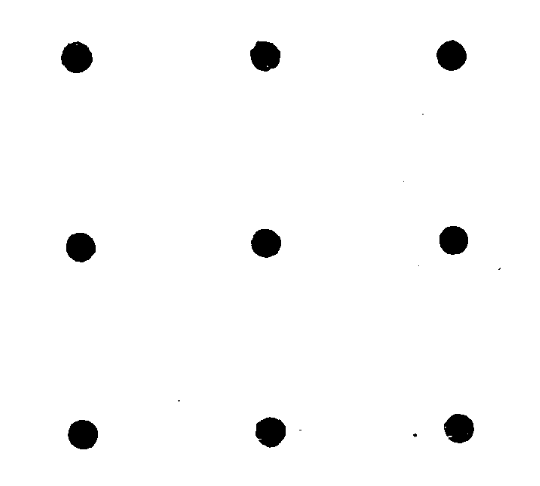
\includegraphics[width=0.5\textwidth]{sdevi_q133.png}
\caption{ Qs 133}
\end{center}
\end{figure}


Can you  draw  four  straight  lines,  the second  beginning where  the first  ends,  the third  beginning  where  the second ends,  and the fourth  beginning  where  the  third  ends  so that each  dot is or at least  one line? 


\item \textbf{LONGFELLOW  AND  HIS  BEES} \\
Here  is a simple  arithmetical  puzzle  set  by  Long-fellow  in his own  flowery,  poetical  language. 

If one-fifth  of a hive  of bees  flew  to the  badamba flower,  one-third  flew  to the  slandbara,  three  times  the difference  of these  two numbers  flew  to an arbour,  and one bee continued  to fly about,  attracted  on each  side  by the fragrant  Ketaki  and Malati,  what  was  the number  of bees? 


\item \textbf{THE  TENNIS  TOURNAMENT} \\
A singles  tennis  tournament  is held  in which  30 men participate.  If a player  is eliminated  as soon  as he loses a match,  how  many  matches  are  required  to determine the winner? 
84 

\item \textbf{THE  TRIANGLES} \\ 
How  many  triangles,  of any size,  are there  in this star: 
\begin{figure}[h]
\begin{center}
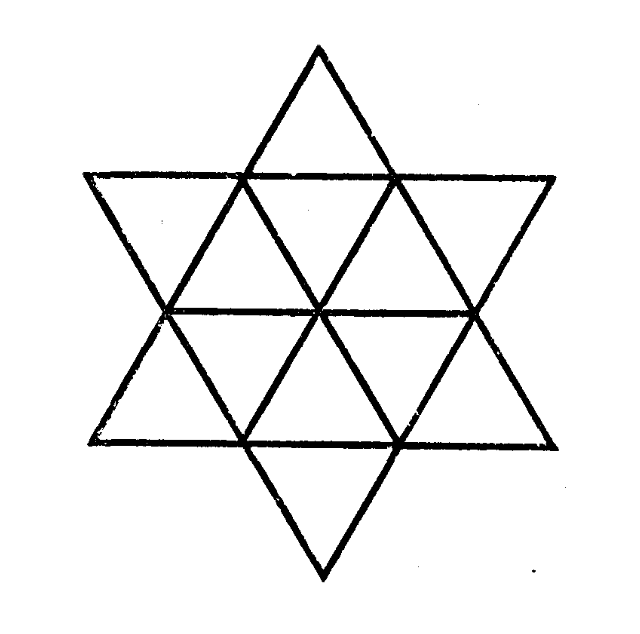
\includegraphics[width=0.5\textwidth]{sdevi_q136.png}
\caption{ Qs 136}
\end{center}
\end{figure}


\item \textbf{DRIVING  THROUGH  THE  COUNTRY} \\ 
I decided  to drive  through  the  country  leisurely,  and on the first  day I did only  7 miles.  On  the last day I did 51 miles,  increasing  my journey  4 miles  each  day. 

How  many  days  did I travel  and how  far? 


\item \textbf{THE  SABBATH  DAY} \\
Christians  hold  the first  day  of the  week  as Sabbath, the Jews  the seventh,  and the Turks  the sixth. 

How  can these  three,  have  each  his own  true  Sabbath on the same  day ? 


\item \textbf{THE  PUZZLED  ARTIST} \\
An artist  wanted  to paint  a picture  on a canvas  which would  allow  for a margin  of 4 inches  on top  and  on bottom  and  two  inches  on each  side.  He  wanted  the picture  itself  to occupy  72 square  inches. 

What  should  be the smallest  dimensions,  the canvas  he is going  to obtain,  should  possess? 


\item \textbf{THE  MYSTERY  OF NUMBER  ELEVEN} \\ 
Can you  find  the  largest  possible  number  containing any 9 of the 10 digits,  considering  O also  as a number, that is divisible  by 1), without  a remainder? 


\item \textbf{THE  ROSE  GARDEN}
In my bungalow  in Bangalore  I have  a beautiful  rose garden. 

The four  sides  of the garden  are known  to be 20,  16, 12 and 10 rods.  And  it is also  known  that  it has  the greatest  possible  area  for those  sides. 

Can you  find  the area? 

\item \textbf{SQUARES  WITHIN  SQUARE} \\ 
In tbe illustrations  below,  how  many  squares  are there? 
\begin{figure}[h]
\begin{center}
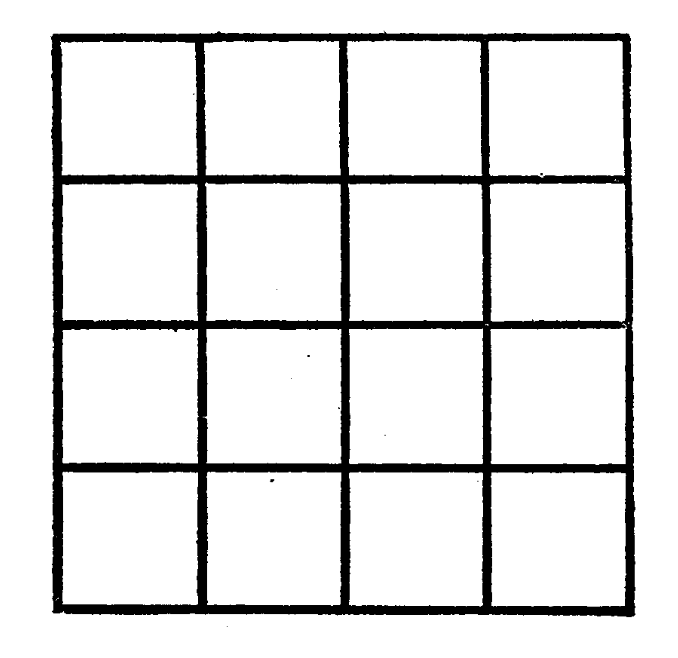
\includegraphics[width=0.5\textwidth]{sdevi_q142.png}
\caption{ Qs 142}
\end{center}
\end{figure}


\item \textbf{THE  FARMER  AND  THE  ANIMALS} \\
Parmer  Thimmayya  bought  some  mules  at Rs.  50 each,  sheep  at Rs.  40 each,  goats  at Rs.  25 each,  and pigs at Rs. 10 each.  The  average  price  of the  animals per head  worked  to Rs. 30. 

How  many  animals  of each  kind  did he buy?

 

\item \textbf{THE  MANGO  THIEVES} \\
One night  three  naughty  boys  stole  a basketful  of mangoes  from  a garden,  hid the  loot  and  went  to sleep. Before  retiring  they  did some  quick  counting  and  found that the fruits  were  less than  a hundred  in number. 

During  the  night  one  thief  awoke,  counted  the mangoes  and found  that  he could  divide  the mangoes  into three  equal  parts  if he first  took  one  for himself.  He  then took  one  mango,  ate it up, and  took  1/3 of the  rest,  hid them  separately  and  went  back  to sleep.

Shortly  thereafter  another  thief  awoke,  counted  the mangoes  and he again  found  that  if he took  one  Cor himself  the loot  could  be divided  into  three  equal  parts. He ate up one mango,  bagged  J of.  the remainder,  hid them  separately  and  went  back  to sleep.  The  third  thief also awoke  after  some  time,  did the same  and  went  back to sleep. 

In the morning  when  they  all woke  up;  and  counted their  mangoes,  they  found  that  the  remaining  mangoes again  totalled  1 more  than  could  be divided  into  three equal  parts. 

How  many  mangoes  did the boys  steal?


\item \textbf{THE  HOUSE  WHERE  SHE  LIVES} \\ 
It was  at a cocktail  party  in New  York  that  I met Stephanie.  We  exchanged  our  phone  numbers  and decided  to meet  each  other  soon. 

When  she rang  up and invited  me to her house  this  is how she gave  me the number  of her hduse: 

'I live in a long  street.  Numbered  on my  side  are the bouses  one,  two,  three  and  so on.  All  the numbers on one side  of me add  up exactly  the  same  as all the numbers  on the other  side  of me. I know  there  are more than fifty  houses  on that  side  of the  street,  but  not  so many  as five  hundred. 

Can you find  Stephaine's  house  number? 


\item \textbf{A MATTER  OF RUPEES  AND  PAISES} \\
I have  a money  pouch  containing  Rs.  700.  There are an equal  number  of 25 paise  coins,  50 paise  coins and one rupee  coins. 

How  many  of each  are there? 


\item \textbf{SAWING  THE  CUBE} \\ 
We have  a wooden  cube  of 3" on a side  and  we  have a buzz-saw.  The  cube  can be cut into  27 one  inch  cubes by the buzz-saw.  Only  6 cuts  of saw are necessary  to do this, while  keeping  the  pieces  together.  Now,  can  you reduce  the number  of cuts  by rearranging  the pieces  after each cut?  If you can,  how  is it done?  If you  can't, why can't  it be done  ? 


\item \textbf{THE  TWO  TRAINS} \\
Two trains  start  at the same  time,  one  from  Bangalore to Mysore  and the other  from  Mysore  to Bangalore.  If they arrive  at their  destinations  one hour  and  four  hours respectively  after  passing  one another,  how  much  faster  is one train  running  than  the other? 
91 

\item \textbf{THE  SQUARES} \\
Can you find  four  numbers  such  that  the  sum  of every two and the sum  of all four  may  be perfect  squares? 


\item \textbf{THE  ARITHMETICAL  LANDLADY} \\
While  house  hunting  in London,  I came  across  a very good  basehold  property.  Discussing  the lease  the  land-lady told  me: 

'The property  was  originally  on a 99 years  lease  and two-thirds  of the time  past  is equal  to four-fifths  of the time to come.  Now  work  it out for yourself  and see how many  years  are there  to go!

How  many  years  of unexpired  lease  did  the property have? 
\end{enumerate}
\end{document}
